\chapter{Modellbildung}

Ein Ziel dieser Arbeit besteht darin, für die am PtU der TU Darmstadt entwickelte und konstruierte 3D-Servo-Presse ein Black-Box-Modell zu entwickeln. Für die Bestimmung der Eingangs- und Ausgangsgrößen für das Modell ist die Erläuterung des Aufbaus und der Funktionsweise der 3D-Servo-Presse notwendig. Daraufhin erfolgt die Modellbildung der 3D-Servo-Presse mittels verschiedener neuronaler Netze. Die entwickelten Modelle werden dann in Bezug auf ihre Approximationsfähigkeit, Trainingszeit, Robustheit, ihr Interpolations- und Extrapolationsverhaltens untersucht.

\section{Aufbau der 3D-Servo-Presse}

Wie in Abbildung \ref{fig:3d-servo} zu erkennen ist, befindet sich das Pressengetriebe im oberen und der Arbeitsbereich mit dem Stößel im unteren Bereich.

\begin{figure} [h]
	\centering
	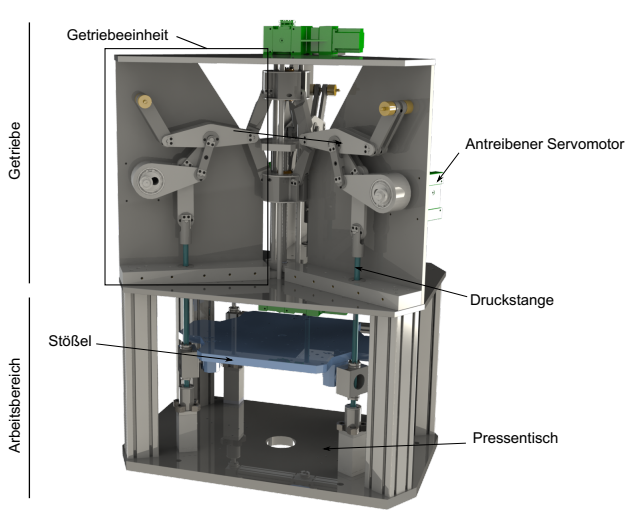
\includegraphics[width=0.75\textwidth]{images/3D-Servo-Presse}
	\caption{Oberer Pressenaufbau der 3D-Servo-Presse mit geöffnetem Getriebekasten \cite{Rakowitsch.2018}}
	\label{fig:3d-servo}
\end{figure}

Das Pressengetriebe besteht aus insgesamt drei Getriebeeinheiten, welche um $120^\circ$ versetzt sind. Der Antrieb jeder Getriebeeinheit erfolgt über einen Servo-Motor, dessen Rotationsbewegung über ein Koppeltriebe in eine translatorische Hubbewegung der zum Getriebe gehörende Druckstange umgesetzt wird, siehe Abbildung \ref{fig:koppel}.

\begin{figure} [h]
	\centering
	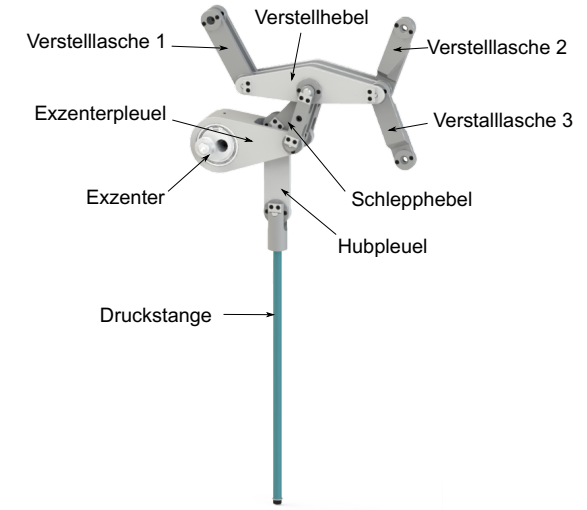
\includegraphics[width=0.65\textwidth]{images/exzenter}
	\caption{Koppelgetriebe mit Getriebeelementen zur Transformation der rotatorischen Bewegung des Servo-Motors in eine Hubbewegung der Druckstange \cite{Rakowitsch.2018}}
	\label{fig:koppel}
\end{figure}


Gelenke verbinden dabei die drei Druckstangen mit dem Stößel. Für eine rein translatorische Hubbewegung des Stößels verfahren alle drei Druckstangen gleichermaßen. Verfahren die drei Druckstangen unterschiedlich, kommt es zu einer Schrägstellung des Stößels. Jede der drei Getriebeeinheiten ist wiederum mit einer sich im Zentrum befindenden Verstelleinheit verbunden, siehe Abbildung, \ref{fig:verstelleinheit}.
\begin{figure} [h]
	\centering
	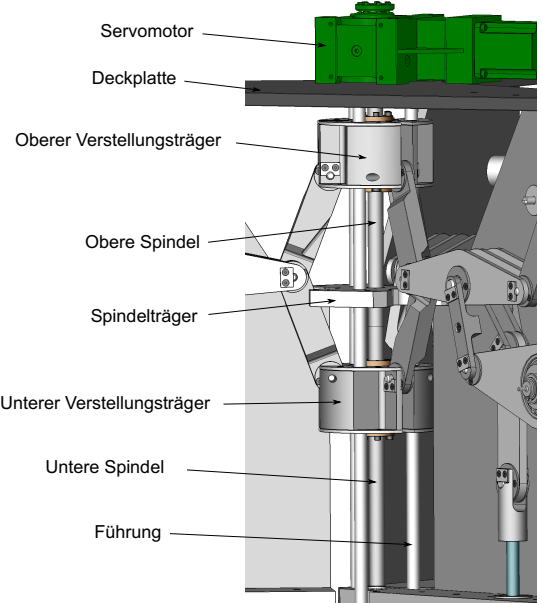
\includegraphics[width=0.6\textwidth]{images/verstelleinheit}
	\caption{Verstelleinheit zur Einstellung des oberen und unteren Totpunktes für die Druckstangen \cite{Rakowitsch.2018}}
	\label{fig:verstelleinheit}
\end{figure}
Die Verstelleinheit besteht aus Führungsstangen und zwei übereinander angeordneten Spindeln, wobei jede Spindel durch Servo-Motor verstellt werden kann. Durch die Verstellung der oberen und der unteren Spindel findet die Einstellung des oberen und des unteren Totpunktes für die Druckstange statt. Die Einstellung des oberen und des unteren Totpunktes gilt dabei für jede Getriebeeinheit, da jede Getriebeeinheit mit der gleichen Verstelleinheit verbunden ist. Die Höhenverstellung jeder der drei Druckstangen ist also bedingt durch die Verstellung der oberen und unteren Spindel, genannt $s_o$ und $s_u$, und durch den Exzenterwinkel $\varphi_{exz}$, siehe Abbildung \ref{fig:prinzipskizze}.

\begin{figure} [h]
	\centering
	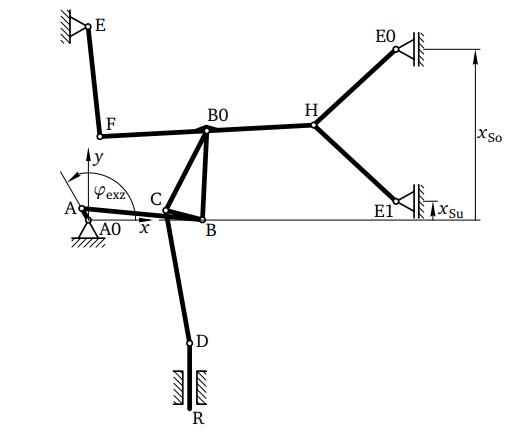
\includegraphics[width=0.65\textwidth]{images/prinzipskizze}
	\caption{Prinzipskizze des Getriebes \cite{Rakowitsch.2018}}
	\label{fig:prinzipskizze}
\end{figure}


Das Pressenmodell wird für eine rein translatorische Bewegung des Stößels entwickelt. Damit ist die Höhenverstellung aller drei Druckstangen identisch. Die Höhenverstellung der drei Druckstangen entspricht somit auch der Höhenverstellung des Stößels. 
Damit ist es zweckmäßig, ein Pressenmodell zu entwickeln, welches die Eingangsgrößen (obere Verstellung der Spindel $s_o$, untere Verstellung der Spindel $s_u$ und der Exzenterwinkel $\varphi_{exz}$) in die Höhenverstellung $y$ des Stößels als Ausgangsgröße transformiert. 





  
  
  
  
  
 
